\section{Results}
\subsection{$\gamma$ spectra of four different sources}
The energy calibration of the MCA was accomplished using the known decay 
schemes (see \autoref{sec:decay_schemes}) of four radioactive sources: 
\cesium, \cobalt, \lead and \hafnium.
Figure \ref{fig:calibration_energy} in \autoref{sec:calibration} 
shows the linear fit and the resulting calibration factor, 
relating the channel number and the energy $E$ expressed in keV.

Once the calibration was performed, it was possible to draw the $\gamma$ spectra 
of the four sources, as depicted in Figure \ref{fig:gamma_spectra}.
Comparing with the decay schemes, their $\gamma$ peaks were identified,
as well as other contributions:
the Compton edge, which appears most notably in the \cesium 
and the \lead spectra, and a peak whose energy matches the $\gamma_1$ peak of \lead,
visible in the \cesium and \hafnium spectra. 
As expected (or detailed in Section \ref{sec:separation}), the $\gamma_2$ and $\gamma_3$ peaks of \cobalt are not distinguishable, due the energetic proximity of these rays.
Only one $\gamma$ peak was detected for \hafnium, of the 4 expected from its decay scheme.

\begin{figure}[htbp]
    \centering
    \begin{subfigure}{0.495\textwidth}
        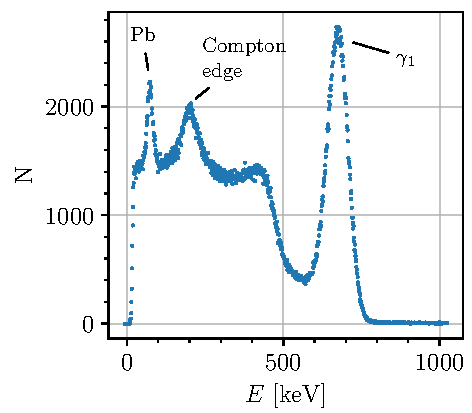
\includegraphics[scale=1]{figures/cs137_spectrum.pdf}
        \caption{}
    \end{subfigure}
    \hfill
    \begin{subfigure}{0.495\textwidth}
        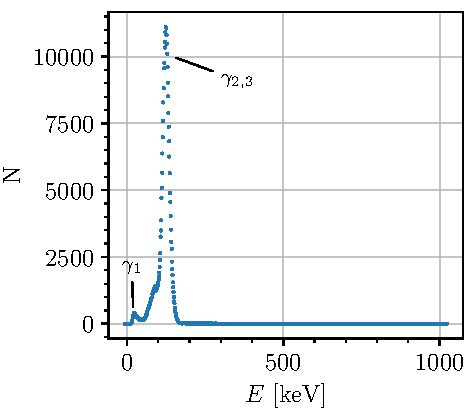
\includegraphics[scale=1]{figures/co57_spectrum.pdf}
        \caption{}
    \end{subfigure}
    \begin{subfigure}{0.495\textwidth}
        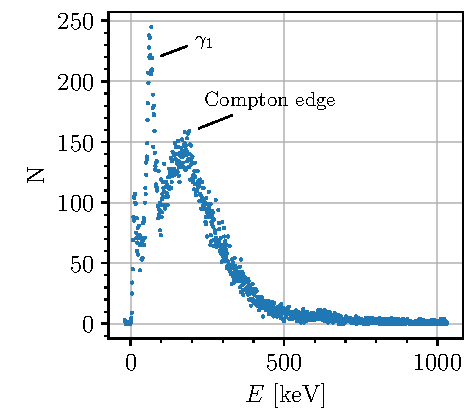
\includegraphics[scale=1]{figures/pb210_spectrum.pdf}
        \caption{}
    \end{subfigure}
    \hfill
    \begin{subfigure}{0.495\textwidth}
        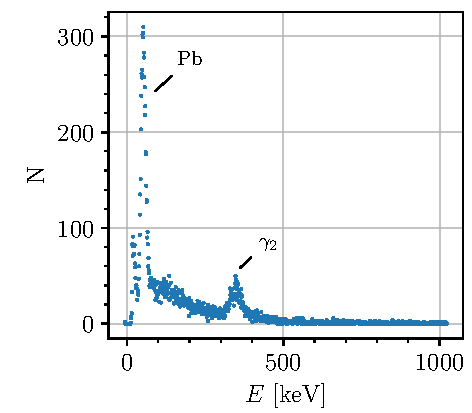
\includegraphics[scale=1]{figures/hf181_spectrum.pdf}
        \caption{}
    \end{subfigure}
    \caption{Gamma spectra of (a) $^{137}$Cs, (b) $^{57}$Co, (c) $^{210}$Pb, (d) $^{181}$Hf.}
    \label{fig:gamma_spectra}
\end{figure}


\subsection{Statistics [TODO relire]}
It was discussed in Section \ref{sec:statistics} that the number of desintegrations detected 
in a fixed interval of time follows a Poisson distribution, which tends to 
a gaussian distribution for a high mean.
To this end, \cesium was used due to its high activity.
To test these assumptions, two sets of measures were taken, using the MCA in MCS mode: 
the first ("Low Mean") with a dwell time of $3$ ms, which gave an average of $m = 2.27$ desintegrations per interval, 
and the second ("High Mean") with a dwell time of $300$ ms, with an average of $m = 228.10$.
Both were compared through Pearson's $\chi^2$ test 
with a Poisson distribution of parameter $\lambda = m$ 
and a gaussian distribution of mean $m$ and standard deviation $\sqrt{m}$.
These test distributions are depicted in \autoref{fig:statistical_tests} with
the respective data sets.
while the results of the statistical tests are summarised in \autoref{tab:statistical_tests}.
%
\begin{figure}[htbp]
    \centering
    \begin{subfigure}{0.495\textwidth}
        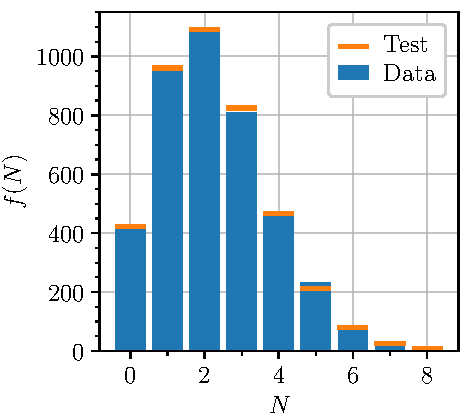
\includegraphics[scale=1]{figures/lowmean_poisson.pdf}
        \caption{}
    \end{subfigure}
    \hfill
    \begin{subfigure}{0.495\textwidth}
        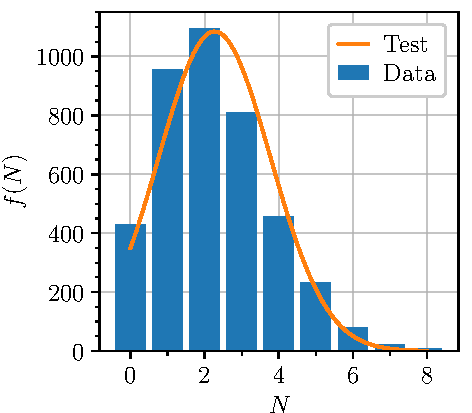
\includegraphics[scale=1]{figures/lowmean_gaussian.pdf}
        \caption{}
    \end{subfigure}
    \begin{subfigure}{0.495\textwidth}
        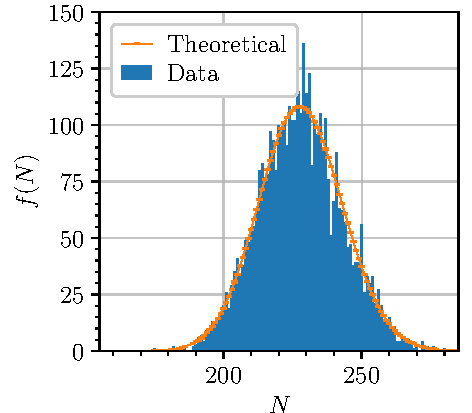
\includegraphics[scale=1]{figures/highmean_poisson.pdf}
        \caption{}
    \end{subfigure}
    \hfill
    \begin{subfigure}{0.495\textwidth}
        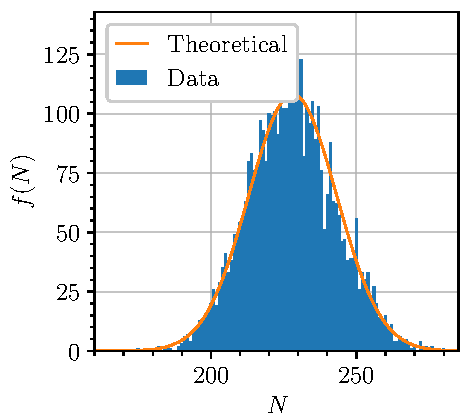
\includegraphics[scale=1]{figures/highmean_gaussian.pdf}
        \caption{}
    \end{subfigure}
    \caption{Frequencies of the number of desintegrations detected 
    in a fixed interval of time, compared with test distributions: 
    (a) Low Mean and Poisson, (b) Low Mean and gaussian, 
    (c) High Mean and Poisson, (d) High Mean and gaussian.
    The error bars on the frequencies were omitted for visibility and in reason of their small size.}
    \label{fig:statistical_tests}
\end{figure}

\begin{table}[htbp]
    \centering
    \begin{tabular}{lllllll}
        \hline
        Data set & Mean & Test distribution & dof & $p$-value & Result \\
        \hline
        \multirow{2}{*}{Low mean} & \multirow{2}{*}{2.27} & Poisson & 8 & 0.86 & Accepted\\
        & & Gaussian & 7 & $5.7 \times 10^{-117}$ & Rejected \\
        \multirow{2}{*}{High mean} & \multirow{2}{*}{228.10} & Poisson & 91 & 0.38 & Accepted\\
        & & Gaussian & 90 & 0.26 & Accepted\\
        \hline
    \end{tabular}
    \caption{Results of the statistical tests carried out on 
    the distribution of the number of desintegrations detected 
    in a fixed interval of time, carried out on two data sets 
    of different mean.}
    \label{tab:statistical_tests}
\end{table}

\subsection{Attenuation in matter}
The study of the attenuation of $\gamma$ rays in matter was conducted using 
a sample of \cesium, a source more suited to the role than 
the others available due to its higher activity.
Measures of the intensity of the radiation were taken for
different widths of aluminium and lead shielding applied 
between the source and the detector.
Figure \ref{fig:attenuation_coefficient} depicts the results obtained with 
the two materials:
the attenuation is exponential in nature, as described 
by Eq.\eqref{eq:attenuation_law}, and more effective using lead than aluminum.
The linear attenuation coefficient of each material was obtained by linear regression, yielding \mbox{$\mu_{\mathrm{Al}} = (0.20 \pm 0.01)$ \unit{\per\cm}} for aluminium
and \mbox{$\mu_{\mathrm{Pb}} = (1.08 \pm 0.03)$ \unit{\per\cm}} for lead.
\begin{figure}[htbp]
    \centering
    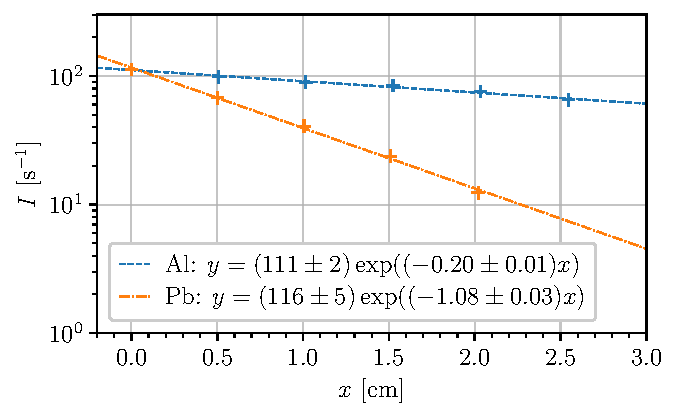
\includegraphics[scale=1]{figures/attenuation_coefficient.pdf}
    \caption{Radiation attenuation through Aluminum (Al) and Lead (Pb). 
             The error bars were omitted in reason of their small relative size 
             (1\% on the intensity and $1$ $\mu$m on the thickness of the material).}
    \label{fig:attenuation_coefficient}
\end{figure}


\subsection{Activity of \cobalt}
The experimental setup for coincidence detection described 
in Section \ref{sec:coincidences} allows for the calculation
of the activity $A$ of the sample of \cobalt.
After determining the time resolution $2\theta$ of 
the instrument, by means of the linear fit depicted in
\autoref{fig:twotheta_cs137}, \autoref{eq:activity} allowed 
to obtain a value of $A= (4120 \pm 50)$ Bq.

\begin{figure}[htbp]
    \centering
    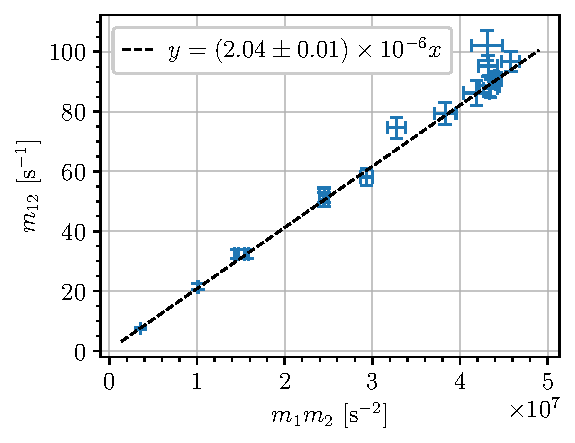
\includegraphics[scale=1]{figures/twotheta_cs137.pdf}
    \caption{Determination of the time resolution of the coincidence
    selector, as described by \autoref{eq:coincidence_time_resolution}.}
    \label{fig:twotheta_cs137}
\end{figure}


\subsection{$\gamma_2$ and $\gamma_3$ peak separation}

Following the setup described in \autoref{sec:separation}, a spectrum containing only the \(\gamma_2\) rays of the \cobalt desintegration was aquired. The spectrum containing only \(\gamma_2\), \(\gamma_3\) were plotted alongside the complete spectrum, shown in \autoref{fig:co57_gamma3_spectrum}. Using a gaussian fit around the separated \(\gamma_2\) and \(\gamma_3\) peaks, the energy of both rays were determined. The energy of the \(\gamma_2\) ray was found to be \(E_{\gamma_2} = (122 \pm 10)\) keV, and the energy of \(\gamma_3\) \(E_{\gamma_3} = (126 \pm 11)\) keV.

\begin{figure}[htbp]
    \centering
    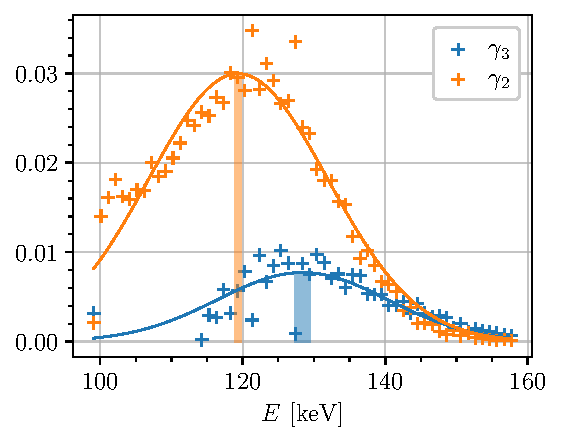
\includegraphics[scale=1]{figures/co57_gamma2_gamma3.pdf}
    \caption{Separated peaks of $\gamma_2$ and $\gamma_3$ rays of \cobalt desintegration and their respective energy.}
    \label{fig:co57_gamma3_spectrum}
\end{figure}

\subsection{Half-life of 14.4 keV excited state}

The recorded delays between a detected \(\gamma_2\) and \(\gamma_1\) ray are shown in \autoref{fig:delay_gamma12}. The linear calibration relationship used for channel to time mapping is shown in \autoref{sec:calibration}. The data was fitted with an exponentially modified Gaussian, in accord with the theory described in \autoref{sec:half_life}, along with a normalisation factor:
\begin{equation}
    f(x;\mu,\sigma,\lambda, N) = \frac{1}{N} \frac{\lambda}{2} e^{\frac{\lambda}{2} (2 \mu + \lambda \sigma^2 - 2 x)}
             \operatorname{erfc} \left(\frac{\mu + \lambda \sigma^2 - x}{ \sqrt{2} \sigma}\right)
\end{equation}
The exponential distribution factor was found to be \(\lambda = 5.94 \pm 0.01\), which yields an estimated half-life of \(t_{1/2} = (116 \pm 1)\) ns for the 14.4 keV excited state.

\begin{figure}[h]
    \centering
    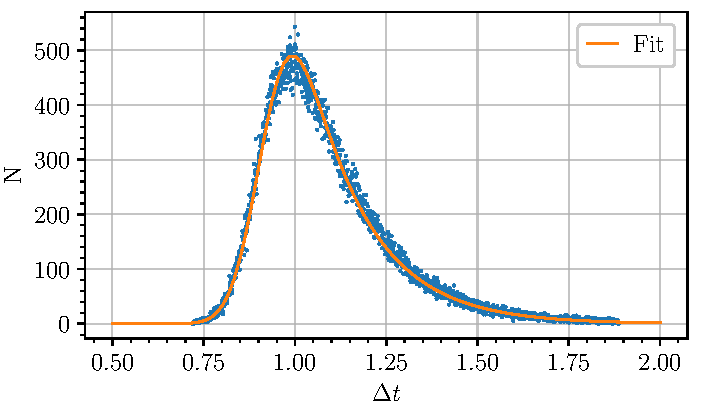
\includegraphics[scale=1]{figures/co57_halflife.pdf}    
    \caption{Distribution of the measured delays between \(\gamma_2\) and \(\gamma_1\) signals.}
    \label{fig:delay_gamma12}
\end{figure}

